% Provenance (never printed): old terminale S material on past climates (ice cores,
% pollen, ocean sediments and oxygen isotopes, glacial-interglacial cycles, the
% astronomical rhythm told, climates of deep time), read from data. Owner (Sync 0/1):
% climate archive and proxy, ice core, glacial period, interglacial and glacial cycle,
% pollen analysis, Last Glacial Maximum. Recalled: glacier, ice sheet, ice age (Book 1,
% grade 8); the first look at the ice-core records (Book 1, grade 9); isotopes
% (physics); greenhouse gases (chemistry); the time scale (Book 1, grade 7). The
% delta notation of isotopes is Book 3's: isotope curves are read here as told,
% without a definition. The orbital theory of climate belongs to a university book:
% told here only. Physical science only, in the IPCC's calibrated words.
% Figures: figdata/grade-12/ice_age_records.py (tests/grade-12/test_ice_age_records.py).
\chapter{अतीत की जलवायु पढ़ना}\label{ch:g12:past-climates}

पूर्वी अंटार्कटिक हिमचादर पर \qty{3233}{m} की ऊँचाई पर स्थित डोम~C में वायु का
वार्षिक औसत तापमान लगभग \qty{-55}{\degreeCelsius} है। वहाँ काम कर रही एक ड्रिल
\qty{3260}{m} की गहराई पर रुकी, बर्फ़ के नीचे की चट्टान से लगभग \qty{15}{m} ऊपर।
उसके द्वारा निकाली गई सबसे गहरी बर्फ़ में वायु के नन्हे बुलबुले हैं जो कोई
\num{800000} वर्ष पुराने हैं: पहले किसानों से बहुत पहले के
वायुमंडल का एक नमूना। यह अध्याय
अतीत की जलवायु को बर्फ़ में, झीलों और समुद्र-तल के
कीचड़ में, और चट्टानों में पढ़ता है, और पूछता है कि वह आज के बारे में क्या कहती है।
% ledger: ipev:concordia, edc3:drilling, jouzel07:edc

\begin{omfigure}
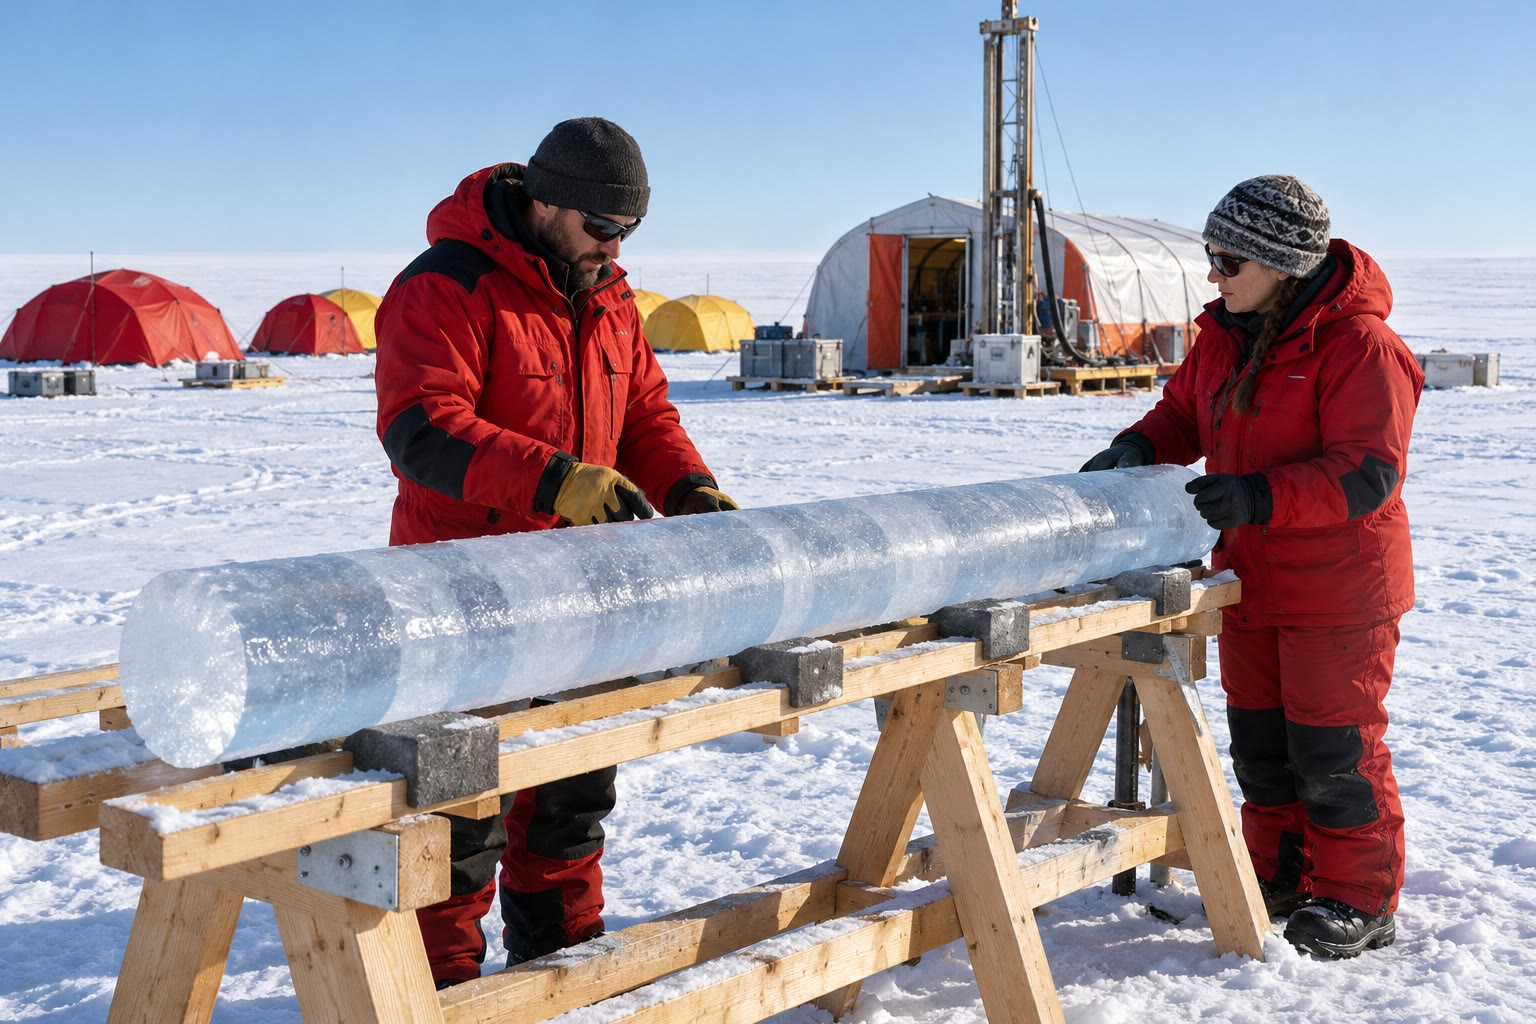
\includegraphics[width=0.56\linewidth]{images/book2/ai/g12-ice-coring-camp.jpg}

{\small किसी ध्रुवीय हिमचादर पर \omterm{def:g12:past-climates:ice-core}{बर्फ़ का कोर} निकालने का एक शिविर: ड्रिल
मीनार और आश्रय के नीचे काम करती है, और कोर की हर लंबाई को प्रयोगशाला तक जाने से पहले
बिछाकर, दर्ज करके और पैक किया जाता है। एआई-जनित चित्रण।}
\end{omfigure}

\begin{recall}
हिमनद बर्फ़ का एक पिंड है जो वर्ष-दर-वर्ष बना रहता है और अपने
भार से बहता है; हिमचादर किसी महाद्वीप के बड़े भाग को ढकती है; हिमयुग
एक लंबा ठंडा समय है जब हिमचादरें ध्रुवों से बहुत दूर तक फैल जाती हैं (पुस्तक 1, कक्षा 8)।
अंटार्कटिका के \omterm{def:g12:past-climates:ice-core}{बर्फ़ के कोरों} में, हिम वायु का तापमान दर्ज करता है और
बुलबुले स्वयं वायु को रखते हैं, और दोनों अभिलेख साथ-साथ उठते और गिरते हैं
(पुस्तक 1, कक्षा 9)। एक ही तत्त्व के परमाणु अपने न्यूट्रॉनों की संख्या में भिन्न हो
सकते हैं: ये समस्थानिक रसायन में एक जैसा व्यवहार करते हैं पर द्रव्यमान में भिन्न होते हैं (भौतिकी
की पुस्तकें)। कार्बन डाइऑक्साइड एक ग्रीनहाउस गैस है (रसायन की पुस्तकें)।
क्वाटरनरी कल्प 2.58 मिलियन वर्ष पहले शुरू हुआ
(पुस्तक 1, कक्षा 7)।
\end{recall}
% ledger: ics:base.Quaternary (shared), nasaeo:o18 (snow poor in heavy isotopes)

\section{अभिलेखागार और प्रॉक्सी}

\num{20000} वर्ष पहले किसी ने वायु का तापमान नहीं मापा। पर
पृथ्वी ने अनजाने में अभिलेख रखे: बर्फ़ और कीचड़ की परतें, सीपियाँ और पेड़ों के
तने, जिनमें से हर एक उस जलवायु के साथ बदला जिसमें वह बना।

\begin{definition}[जलवायु अभिलेखागार; प्रॉक्सी]\label{def:g12:past-climates:proxy}
\emph{जलवायु अभिलेखागार}\index{जलवायु अभिलेखागार} परतों में, एक के बाद एक,
निक्षेपित कोई प्राकृतिक पदार्थ है जो अपने बनने के समय की जलवायु का चिह्न
रखता है: ध्रुवीय बर्फ़, झीलों और समुद्र-तल के अवसाद, पेड़ों के
वलय, प्रवाल, गुफा-निक्षेप। \emph{प्रॉक्सी}\index{प्रॉक्सी} किसी अभिलेखागार में मापी गई
वह राशि है जो किसी ऐसे जलवायु-चर का स्थान लेती है जिसे
मापा नहीं गया था: वायु के तापमान के लिए पुराने हिम में भारी समस्थानिकों का
अंश, वनस्पति के लिए, और इसलिए जलवायु के लिए,
झील के कीचड़ में हर प्रकार के पराग का अंश।
\end{definition}
% ledger: ncei:proxy, ncei:pollen, nasaeo:o18

\begin{center}
\small
\begin{tabular}{|l|l|l|}
\hline
\textbf{अभिलेखागार} & \textbf{\omterm{def:g12:past-climates:proxy}{प्रॉक्सी}} & \textbf{किसके बारे में बताता है} \\
\hline
ध्रुवीय बर्फ़ & बर्फ़ के भारी समस्थानिक & बर्फ़ के ऊपर वायु का तापमान \\
 & बुलबुलों की वायु & कार्बन डाइऑक्साइड, मीथेन \\
झील के अवसाद, पीट & पराग & वनस्पति, फिर जलवायु \\
समुद्री अवसाद & सीपियों के ऑक्सीजन समस्थानिक & बर्फ़ का आयतन, गहरे जल का तापमान \\
वृक्ष-वलय & वलय की चौड़ाई & वृद्धि की परिस्थितियाँ, वर्ष-दर-वर्ष \\
प्रवाल, गुफा-निक्षेप & समस्थानिक, वृद्धि-पट्टियाँ & समुद्र या वायु का तापमान, वर्षा \\
\hline
\end{tabular}

\medskip
{\small मुख्य \omterm{def:g12:past-climates:proxy}{जलवायु अभिलेखागार} और उनके कुछ \omterm{def:g12:past-climates:proxy}{प्रॉक्सी}।}
\end{center}
% ledger: ncei:proxy, nasaeo:o18

हर \omterm{def:g12:past-climates:proxy}{प्रॉक्सी} को पढ़े जाने से पहले दो चीज़ें चाहिए। उसे एक \emph{घड़ी} चाहिए:
हर परत की आयु, जहाँ वार्षिक परतें दिखती हैं वहाँ उन्हें गिनकर,
रेडियोमितीय काल-निर्धारण से (\cref{ch:g12:age-of-the-earth}), या
अभिलेख को पहले से काल-निर्धारित किसी दूसरे अभिलेख से मिलाकर। और उसे एक \emph{अंशांकन} चाहिए:
मापी गई चीज़ और जलवायु-चर के बीच का संबंध, जो आज ज्ञात किया जाता है, जहाँ
दोनों को एक साथ मापा जा सकता है।

\begin{method}[किसी प्रॉक्सी अभिलेख को पढ़ना]
\begin{enumerate}
  \item अभिलेखागार और \omterm{def:g12:past-climates:proxy}{प्रॉक्सी} पहचानिए: क्या मापा गया, और किसमें?
  \item पता कीजिए कि अक्ष पर समय किस ओर चलता है, और किस इकाई में; जाँचिए
        कि \omterm{def:g12:past-climates:proxy}{प्रॉक्सी} का अक्ष उलटा तो नहीं है।
  \item \omterm{def:g12:past-climates:proxy}{प्रॉक्सी} का अर्थ निकालिए: क्या ऊँचे मान का अर्थ अधिक गरम है या अधिक ठंडा,
        अधिक बर्फ़ या कम?
  \item नमूनों के अंतराल पर ध्यान दीजिए: जिस अभिलेख के बिंदु
        \num{2000} वर्ष के अंतर पर हों, वह एक शताब्दी तक चले परिवर्तन को नहीं दिखा सकता।
  \item पूछी गई तिथियों पर मान, या किसी अंतराल पर माध्य, पढ़िए,
        और परिवर्तन और दरें परिकलित कीजिए।
  \item बताइए कि अभिलेख अपने स्थल पर क्या दिखाता है, और उसके बाद ही यह कि क्या वह
        पूरी पृथ्वी के लिए बोलता है।
\end{enumerate}
\end{method}

\section{बर्फ़ के कोर}

\begin{definition}[बर्फ़ का कोर]\label{def:g12:past-climates:ice-core}
\emph{बर्फ़ का कोर}\index{बर्फ़ का कोर} किसी हिमचादर या हिमनद से ड्रिल करके
निकाला गया बर्फ़ का एक बेलन है। उसकी गहराई बर्फ़ की आयु देती है, जितनी गहरी उतनी पुरानी;
बर्फ़ उस वायु का तापमान दर्ज करती है जिसमें उसका हिम गिरा, और उसके
बुलबुले उस समय की वायु के नमूने रखते हैं।
\end{definition}
% ledger: ncei:proxy, jouzel07:edc

ताज़ा हिम अधिकतर वायु है। अगले वर्षों के हिम के नीचे दबकर, वह
\emph{फ़िर्न} में दब जाता है, एक संहत हिम जिसके छिद्र अब भी वायु को गुज़रने देते हैं।
लगभग 820 से \qty{830}{kg/m^3} के घनत्व पर, जो 50 से \qty{120}{m}
नीचे पहुँचता है, छिद्र बंद हो जाते हैं और वायु बुलबुलों में बंद हो जाती है। इसलिए बर्फ़ दो भिन्न
अभिलेख रखती है। बुलबुलों की वायु वायुमंडल का एक नमूना है, जिसकी कार्बन
डाइऑक्साइड और मीथेन प्रयोगशाला में मापी जाती हैं। स्वयं बर्फ़ तापमान
रखती है: जिन जल-अणुओं में कोई भारी समस्थानिक (ड्यूटेरियम या
ऑक्सीजन-18) होता है, वे हल्के अणुओं की अपेक्षा अधिक आसानी से संघनित होते हैं, इसलिए ध्रुव
की ओर रास्ते में वायु जितनी ठंडी, हिम भारी समस्थानिकों में उतना ही निर्धन होता जाता है।
% ledger: firn:close-off, nasaeo:o18

\begin{omfigure}
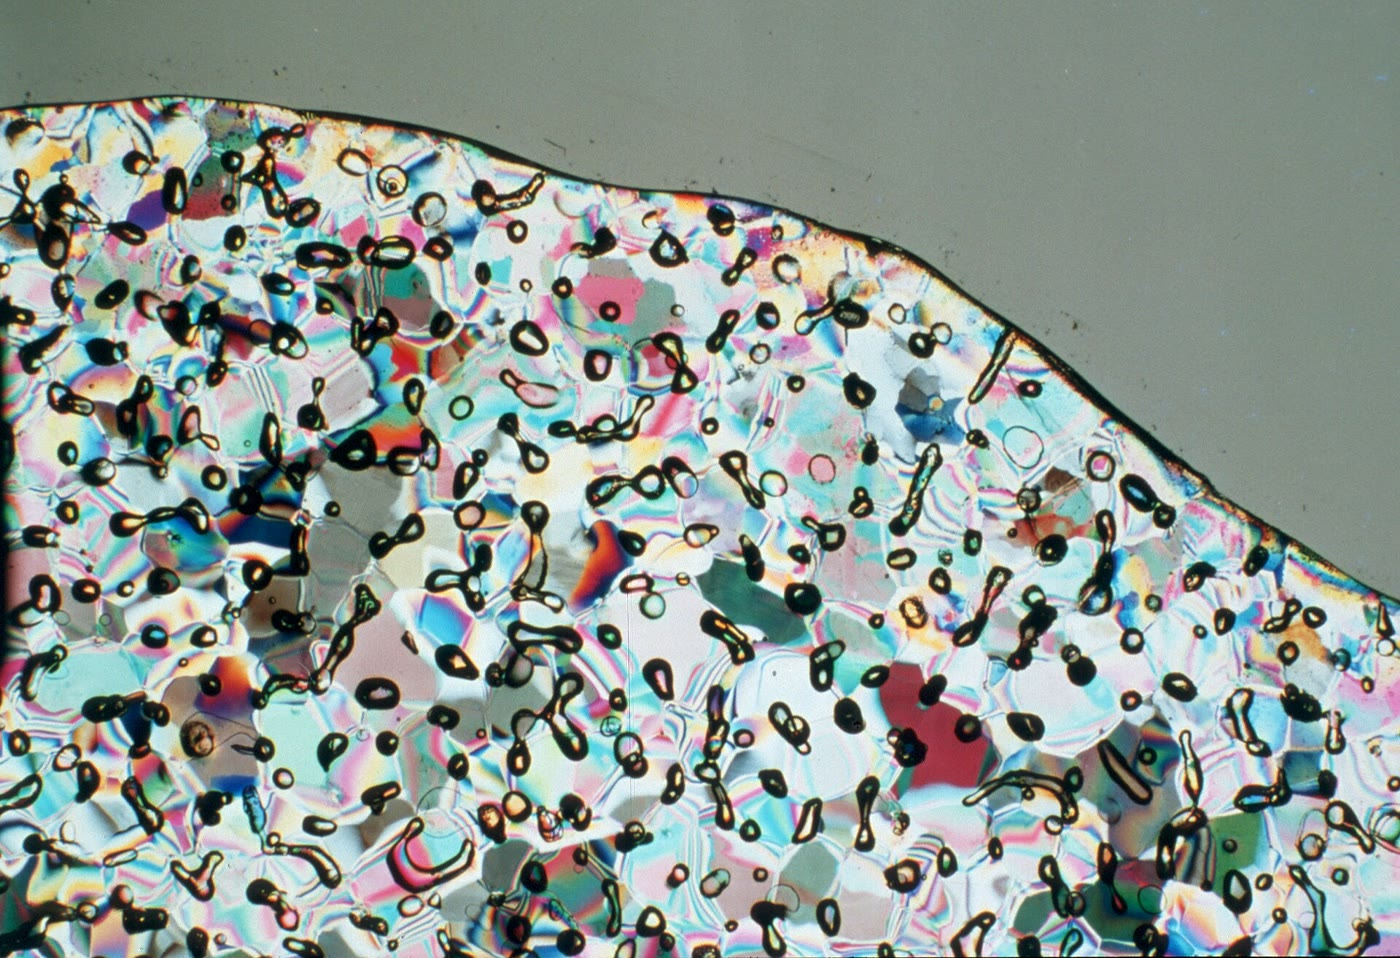
\includegraphics[width=0.50\linewidth]{images/book2/g12-ice-bubbles.jpg}

{\small ध्रुवित प्रकाश में देखी गई अंटार्कटिक बर्फ़ की एक पतली परत, जो बर्फ़ के
क्रिस्टलों को रंग देता है: काले बिंदु फँसी हुई वायु के बुलबुले हैं। फ़ोटो CSIRO
वायुमंडलीय अनुसंधान, CC~BY~3.0 (विकिमीडिया कॉमन्स)।}
\end{omfigure}
% ledger: photo:g12-ice-bubbles

डोम~C कोर के ड्यूटेरियम को बर्फ़ के ऊपर के तापमान में बदला गया है,
जो पिछले हज़ार वर्षों के माध्य की तुलना में परिवर्तन के रूप में दिया गया है।
कार्बन डाइऑक्साइड कई अंटार्कटिक कोरों के बुलबुलों से आती है, जिन्हें
जोड़कर एक अभिलेख बनाया गया है। दोनों नीचे एक ही समय-अक्ष पर खींचे गए हैं।

\begin{omfigure}
\begin{tikzpicture}
\begin{axis}[omrecord, scale only axis, width=0.74\linewidth, height=4.8cm,
  xmin=0, xmax=800, x dir=reverse, ymin=-12, ymax=8, axis y line*=left,
  xtick={0,100,...,800}, ytick={-10,-5,0,5},
  xlabel={1950 से पहले के हज़ार वर्ष},
  ylabel={तापमान-परिवर्तन (\unit{\degreeCelsius})}]
% data:edc-jouzel, 2-kyr means (figdata/grade-12/ice_age_records.py)
\addplot[omWarm, line width=0.7pt] table[x=age_kyr, y=temp_C] {figdata/out/grade-12-ice_age_records-edc.dat};
\end{axis}
\begin{axis}[scale only axis, width=0.74\linewidth, height=4.8cm,
  xmin=0, xmax=800, x dir=reverse, ymin=60, ymax=320, axis y line*=right,
  axis x line=none, ytick={180,220,260,300}, ylabel={कार्बन डाइऑक्साइड (ppm)},
  every axis label/.append style={font=\small}, tick label style={font=\small}]
% data:co2-bereiter, 2-kyr means
\addplot[black, line width=0.7pt] table[x=age_kyr, y=co2_ppm] {figdata/out/grade-12-ice_age_records-co2.dat};
\coordinate (lt) at (axis cs:560,70);
\coordinate (lc) at (axis cs:560,312);
\end{axis}
\node[font=\scriptsize, text=omWarm, anchor=south] at (lt) {डोम~C पर तापमान (बायाँ पैमाना)};
\node[font=\scriptsize, anchor=north] at (lc) {कार्बन डाइऑक्साइड (दायाँ पैमाना)};
\end{tikzpicture}

{\small अंटार्कटिक बर्फ़ के आठ लाख वर्ष, \num{2000} वर्ष के चरणों पर
औसत किए गए। लाल: पिछले हज़ार वर्षों की तुलना में डोम~C पर
तापमान (जूज़ेल और अन्य, 2007); काला: बुलबुलों की
कार्बन डाइऑक्साइड (बेराइटर और अन्य, 2015)। आज दाईं ओर है।}
\end{omfigure}
% ledger: data:edc-jouzel, data:co2-bereiter

दोनों वक्रों का एक ही प्रतिरूप है: दसियों हज़ार वर्षों में ठंड की ओर एक धीमी,
ऊबड़-खाबड़ फिसलन, फिर गरमी की ओर एक तेज़ वापसी, और फिर
से फिसलन।

\begin{definition}[हिमनदीय काल; अंतर्हिमनदीय काल; हिमनदीय चक्र]\label{def:g12:past-climates:glacial-cycle}
\emph{हिमनदीय काल}\index{हिमनदीय काल} किसी हिमयुग के भीतर एक ठंडा अंतराल
है, जिसके दौरान हिमचादरें अपने वर्तमान आकार से बहुत आगे तक बढ़ जाती हैं।
\emph{अंतर्हिमनदीय काल}\index{अंतर्हिमनदीय काल} दो हिमनदीय कालों के बीच
एक गरम अंतराल है, जिसमें हिमचादरें आज जितनी या उससे छोटी होती हैं; हम ऐसे ही एक काल में रहते हैं,
जो लगभग \num{11000} वर्ष पहले शुरू हुआ। \emph{हिमनदीय
चक्र}\index{हिमनदीय चक्र} एक हिमनदीय काल और उसे समाप्त करने वाला
अंतर्हिमनदीय काल है।
\end{definition}
% ledger: ipcc:ref-periods (LDT ends 11 ka); the count of cycles is read from the figure (data:edc-jouzel)

पूरे अभिलेख में, डोम~C पर तापमान
\qty{-10.6}{\degreeCelsius} से, लगभग \num{24000} वर्ष पहले, लेकर
\qty{+5.5}{\degreeCelsius} तक, लगभग \num{129000} वर्ष पहले, बदलता है; कार्बन डाइऑक्साइड
\qty{174}{ppm} से \qty{299}{ppm} तक। \num{2000} वर्षों पर औसत किया गया चित्र
इन चरम मानों को थोड़ा समतल कर देता है। गरम शिखरों की गिनती आठ
या नौ \omterm{def:g12:past-climates:glacial-cycle}{हिमनदीय चक्र} देती है, और तापमान-अभिलेख की सबसे प्रबल लय,
उसके आँकड़ों से परिकलित, का आवर्तकाल लगभग \num{98000} वर्ष है।
% ledger: data:edc-jouzel, data:co2-bereiter (ice_age_records.py: edc_min_C -10.58 at 24.0 kyr, edc_max_C 5.46 at 128.7 kyr, co2 173.71 and 298.6, edc_period_kyr 97.5)

\begin{proposition}[तापमान और कार्बन डाइऑक्साइड साथ-साथ बदलते हैं]\label{prop:g12:past-climates:correlation}
% ledger: data:edc-jouzel, data:co2-bereiter (ice_age_records.py: r_temp_co2 0.9165, fit 266.57 + 7.827 T, 1639 pairs)
पिछले \num{800000} वर्षों में, अंटार्कटिक तापमान और वायु की कार्बन
डाइऑक्साइड साथ-साथ बदले। \num{2000} वर्ष से पुराने 1639 कार्बन डाइऑक्साइड
मापनों में से हर एक को उसी आयु के डोम~C तापमान के साथ
जोड़ने पर सहसंबंध गुणांक $r = 0.92$ मिलता है, और
न्यूनतम-वर्ग रेखा
\[
  \mathrm{CO_2} \approx \qty{267}{ppm} + \qty{7.8}{ppm/\degreeCelsius} \times \Delta T ,
\]
जहाँ $\Delta T$ डोम~C पर तापमान-परिवर्तन है।
\end{proposition}

\begin{proof}[इसे कैसे परिकलित किया जाता है]
हर कार्बन डाइऑक्साइड नमूने के लिए, उसकी आयु पर तापमान
डोम~C अभिलेख में दो निकटतम तापमान-बिंदुओं के बीच अंतर्वेशन करके पढ़ा जाता है।
1639 जोड़ों का सहसंबंध गुणांक, $-1$ और $1$ के बीच की एक संख्या
जो मापती है कि बिंदु किसी सीधी रेखा के कितने निकट हैं (गणित की
पुस्तकें), न्यूनतम-वर्ग रेखा के साथ परिकलित किया जाता है; दोनों
चित्र की स्क्रिप्ट में परिकलित होते हैं और उसके परीक्षण द्वारा जाँचे जाते हैं।
\end{proof}

\begin{omfigure}
\begin{tikzpicture}
\begin{axis}[omrecord, width=0.70\linewidth, height=5.2cm, xmin=-12, xmax=6,
  ymin=160, ymax=310, xlabel={डोम~C पर तापमान-परिवर्तन (\unit{\degreeCelsius})},
  ylabel={कार्बन डाइऑक्साइड (ppm)}]
% data:edc-jouzel, data:co2-bereiter (pairs and fit in ice_age_records.py)
\addplot[only marks, mark=*, mark size=0.6pt, omDef, opacity=0.45] table[x=temp_C, y=co2_ppm] {figdata/out/grade-12-ice_age_records-pairs.dat};
\addplot[omThm, line width=1pt] table[x=temp_C, y=co2_ppm] {figdata/out/grade-12-ice_age_records-fit.dat};
\node[font=\scriptsize, text=omThm, anchor=south east, fill=white, inner sep=1pt] at (axis cs:-1.5,295) {न्यूनतम-वर्ग रेखा, $r = 0.92$};
\end{axis}
\end{tikzpicture}

{\small हर बिंदु अंटार्कटिक बर्फ़ का एक कार्बन डाइऑक्साइड मापन है,
जिसे उसी आयु के डोम~C तापमान पर रखा गया है: ठंडे युगों में कार्बन
डाइऑक्साइड कम थी, गरम युगों में कहीं अधिक। जूज़ेल और अन्य (2007) और
बेराइटर और अन्य (2015) से परिकलित।}
\end{omfigure}

सहसंबंध यह नहीं बताता कि पहले कौन बदला, न यह कि किसी तीसरे कारण ने
दोनों को हिलाया: गुणांक वही होता यदि तापमान कार्बन डाइऑक्साइड को चलाता,
यदि कार्बन डाइऑक्साइड तापमान को चलाती, या यदि हर एक दूसरे को धकेलता।
लगभग \num{100000} वर्ष की लय को क्या तय करता है, यह नीचे महासागर वाले
खंड में बताया गया है, और कार्बन डाइऑक्साइड तापमान पर कैसे काम करती है, यह
\cref{ch:g12:climate-change} में।

\subsection{अंतिम हिमनदीय अधिकतम}

\begin{definition}[अंतिम हिमनदीय अधिकतम]\label{def:g12:past-climates:lgm}
\emph{अंतिम हिमनदीय अधिकतम}\index{अंतिम हिमनदीय अधिकतम} वह समय है, लगभग
\num{23000} से \num{19000} वर्ष पहले, जब पिछले \omterm{def:g12:past-climates:glacial-cycle}{हिमनदीय
काल} की हिमचादरें अपने सबसे बड़े आकार पर थीं।
\end{definition}
% ledger: ipcc:ref-periods

\omterm{def:g12:past-climates:lgm}{अंतिम हिमनदीय अधिकतम} पर, हिमचादरें उत्तरी अमेरिका और
उत्तर-पश्चिमी यूरेशिया के बड़े भाग को ढके हुए थीं, और जलवायु आज से अधिक शुष्क और धूल-भरी थी।
आकलनों का अनुमान है कि वैश्विक सतह-तापमान 1850--1900 की तुलना में \qty{5}{\degreeCelsius}
से \qty{7}{\degreeCelsius} कम था (\emph{मध्यम विश्वास}),
और कार्बन डाइऑक्साइड 188 से \qty{194}{ppm} थी। हिमचादरों में बंद
जल महासागर से आया था: वैश्विक माध्य समुद्र-तल आज से 125 से \qty{134}{m}
नीचे था।
% ledger: ipcc:ref-periods, ipcc:lgm-cooling, ipcc:fig2-34, ipcc:lgm-sea, lambeck14:lgm

नीचा समुद्र महाद्वीपों के चारों ओर के उथले तल को उघाड़ देता है। नीचे का मानचित्र
समुद्र को \qty{130}{m} नीचे करता है, जो उस परास का मध्य है, दक्षिण-पूर्व एशिया के
उस तल पर जैसा वह आज है।

\begin{omfigure}
\begin{tikzpicture}
\begin{axis}[omrecord, axis equal image, width=0.62\linewidth, xmin=92, xmax=122,
  ymin=-11, ymax=24, grid=none, axis x line=box, axis y line=box,
  xtick={95,105,115}, ytick={-10,-5,...,20},
  xticklabel={\pgfmathprintnumber{\tick}\textdegree पू},
  yticklabels={10\textdegree द, 5\textdegree द, 0\textdegree, 5\textdegree उ, 10\textdegree उ, 15\textdegree उ, 20\textdegree उ}]
% data:b2-etopo-sunda (raster computed in ice_age_records.py; sea level lowered by 130 m)
\addplot graphics[xmin=91.95, xmax=122.05, ymin=-11.05, ymax=24.05] {figdata/out/grade-12-ice_age_records-sunda.png};
\node[font=\scriptsize] at (axis cs:114.5,0.5) {बोर्नियो};
\node[font=\scriptsize, rotate=-45] at (axis cs:101.9,-1.3) {सुमात्रा};
\node[font=\scriptsize] at (axis cs:110.5,-8.6) {जावा};
\node[font=\scriptsize, rotate=-60] at (axis cs:102.2,4.0) {मलय प्रायद्वीप};
\node[font=\scriptsize] at (axis cs:103,16.5) {हिंदचीन};
\node[font=\scriptsize, align=center] at (axis cs:106.5,3.5) {सुंडा\\शेल्फ़};
\node[font=\scriptsize, align=center] at (axis cs:114.5,13) {दक्षिण चीन\\सागर};
\node[font=\scriptsize, align=center] at (axis cs:96,-6) {हिंद\\महासागर};
\end{axis}
\end{tikzpicture}

{\small आज से \qty{130}{m} नीचे समुद्र के साथ दक्षिण-पूर्व एशिया। हरा:
आज की भूमि; भूरा-पीला: वह तल जिसे \qty{130}{m} नीचा समुद्र-तल उघाड़ देता है; नीला:
समुद्र। वर्तमान उच्चावच का उपयोग किया गया है, इसलिए तटरेखा केवल अनुमानित है।
ETOPO1 उच्चावच (NOAA) से, हर 0.1 डिग्री पर परिकलित।}
\end{omfigure}
% ledger: data:b2-etopo-sunda, ipcc:lgm-sea

बोर्नियो, सुमात्रा और जावा मलय प्रायद्वीप और
हिंदचीन के साथ एक ही भूमि बन जाते हैं: सुंडा शेल्फ़, जो आज एक उथले समुद्र के नीचे है, सूखी भूमि थी। मानचित्र पर,
केवल लगभग \qty{36}{m} की गिरावट बोर्नियो को एशिया से जोड़ने के लिए पर्याप्त है, और सुमात्रा और
जावा उससे पहले ही जुड़ जाते हैं। मानचित्र पर,
समुद्र के ऊपर की भूमि 4.11 से बढ़कर 7.16 मिलियन वर्ग किलोमीटर हो जाती है,
1.74 गुना। पूरी पृथ्वी पर, वही \qty{130}{m} की गिरावट
समुद्र के ऊपर की सतह का अंश \qty{29.0}{\percent} से
\qty{33.5}{\percent} कर देती है, लगभग 23 मिलियन वर्ग किलोमीटर नई भूमि।
% ledger: data:b2-etopo-sunda, data:etopo1 (ice_age_records.py: borneo_link_m -36; sunda_land_now_km2 4.105e6, lgm 7.161e6, ratio 1.744; world_land_now_frac 0.2904, lgm 0.3352, world_gain_km2 2.285e7)

\begin{example}[अंतिम विहिमनदन]
\omterm{def:g12:past-climates:lgm}{अंतिम हिमनदीय अधिकतम} के बाद आए तापन को अंतिम
विहिमनदन संक्रमण कहते हैं; आकलन उसे लगभग \num{18000} और
\num{11000} वर्ष पहले के बीच रखते हैं। डोम~C अभिलेख में,
\omterm{def:g12:past-climates:lgm}{अंतिम हिमनदीय अधिकतम} (\num{23000} से \num{19000} वर्ष पहले) का माध्य तापमान
\qty{-9.4}{\degreeCelsius} है; उसके बाद के अंतराल, \num{11000} से
\num{9000} वर्ष पहले, का माध्य \qty{-0.4}{\degreeCelsius} है। अंटार्कटिका के ऊपर की वायु
\qty{9.0}{\degreeCelsius} गरम हुई, जबकि उसकी कार्बन डाइऑक्साइड
\qty{190}{ppm} से \qty{264}{ppm} तक, \qty{74}{ppm} बढ़ी। पूरी पृथ्वी पर,
तापन 5 से \qty{7}{\degreeCelsius} का आकलित शीतलन था, लगभग
\qty{6}{\degreeCelsius}, जो संक्रमण के \num{7000} वर्षों में फैला था:
\[
  \frac{\qty{6}{\degreeCelsius}}{\num{7000}\ \text{वर्ष}} \approx
  \qty{0.86}{\degreeCelsius} \text{ प्रति हज़ार वर्ष।}
\]
इस बीच समुद्र-तल लगभग \qty{-120}{m} से \qty{-50}{m} तक उठा, औसतन लगभग
\qty{10}{mm} प्रति वर्ष।
\end{example}
% ledger: ipcc:ref-periods, ipcc:lgm-cooling, ipcc:lgm-sea, data:edc-jouzel, data:co2-bereiter (ice_age_records.py: edc_lgm_C -9.389, edc_holo_C -0.360, rise 9.029; co2 189.67, 264.10, rise 74.43; ldt_mean_rate 0.857)

\begin{omfigure}
\begin{tikzpicture}
\begin{axis}[omrecord, scale only axis, width=0.74\linewidth, height=4.6cm,
  xmin=0, xmax=30, x dir=reverse, ymin=-11, ymax=12, axis y line*=left,
  xtick={0,5,...,30}, ytick={-10,-5,0},
  xlabel={1950 से पहले के हज़ार वर्ष},
  ylabel={तापमान-परिवर्तन (\unit{\degreeCelsius})}]
\fill[omDef!10] (axis cs:23,-11) rectangle (axis cs:19,12);
\fill[omProp!12] (axis cs:18,-11) rectangle (axis cs:11,12);
% data:edc-jouzel, every sample
\addplot[omWarm, line width=0.6pt] table[x=age_kyr, y=temp_C] {figdata/out/grade-12-ice_age_records-edc30.dat};
\coordinate (lgm) at (axis cs:21,11.6);
\coordinate (ldt) at (axis cs:14.5,11.6);
\coordinate (lt) at (axis cs:5.5,-3.6);
\end{axis}
\begin{axis}[scale only axis, width=0.74\linewidth, height=4.6cm,
  xmin=0, xmax=30, x dir=reverse, ymin=60, ymax=290, axis y line*=right,
  axis x line=none, ytick={200,240,280}, ylabel={कार्बन डाइऑक्साइड (ppm)},
  every axis label/.append style={font=\small}, tick label style={font=\small}]
% data:co2-bereiter, every sample
\addplot[black, line width=0.6pt, mark=*, mark size=0.5pt] table[x=age_kyr, y=co2_ppm] {figdata/out/grade-12-ice_age_records-co230.dat};
\coordinate (lc) at (axis cs:26.5,196);
\end{axis}
\node[font=\scriptsize, anchor=north, align=center] at (lgm) {अंतिम हिमनदीय\\अधिकतम};
\node[font=\scriptsize, anchor=north, align=center] at (ldt) {अंतिम विहिमनदन\\संक्रमण};
\node[font=\scriptsize, text=omWarm, anchor=north] at (lt) {तापमान (बायाँ)};
\node[font=\scriptsize, anchor=south] at (lc) {कार्बन डाइऑक्साइड (दायाँ)};
\end{tikzpicture}

{\small डोम~C पर पिछले \num{30000} वर्ष, हर मापन: तापमान
(लाल) और कार्बन डाइऑक्साइड (काला) \omterm{def:g12:past-climates:lgm}{अंतिम हिमनदीय अधिकतम} से
साथ-साथ ऊपर चढ़ते हैं। छायांकित: IPCC द्वारा काल-निर्धारित \omterm{def:g12:past-climates:lgm}{अंतिम हिमनदीय अधिकतम} और अंतिम विहिमनदन
संक्रमण। आँकड़े: जूज़ेल और अन्य (2007), बेराइटर और
अन्य (2015)।}
\end{omfigure}
% ledger: data:edc-jouzel, data:co2-bereiter, ipcc:ref-periods

\section{पराग}

हर वसंत में पौधे पराग के बादल छोड़ते हैं। उसका अधिकांश भाग खो जाता है, पर कुछ
झीलों और दलदलों पर गिरता है, डूबता है, और कीचड़ में दब जाता है, जहाँ वह
आसपास उगी वनस्पति का अभिलेख रखता है। और हर प्रकार के
पौधे के कणों का अपना आकार और माप होता है।
% ledger: ncei:pollen

\begin{omfigure}
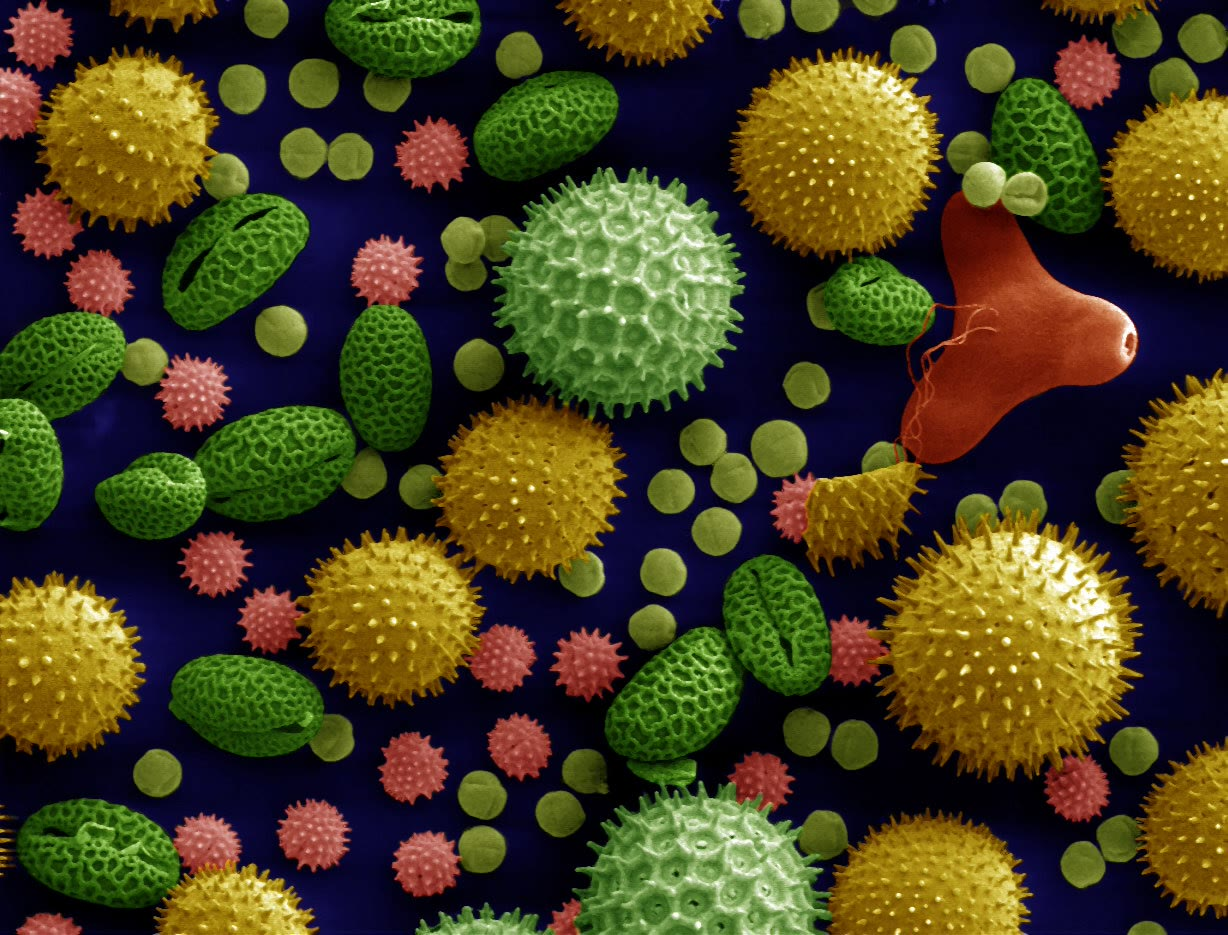
\includegraphics[width=0.46\linewidth]{images/book2/g12-pollen-sem.jpg}

{\small पाँच आम पौधों (सूरजमुखी, नीलकलमी,
गुलखैरा, लिली और प्रिमरोज़) के पराग-कण, क्रमवीक्षण इलेक्ट्रॉन सूक्ष्मदर्शी से
आभासी रंगों में देखे गए। हर प्रकार के पौधे के कण की अपनी आकृति होती है। डार्टमाउथ
इलेक्ट्रॉन सूक्ष्मदर्शी सुविधा (सार्वजनिक डोमेन, विकिमीडिया कॉमन्स के ज़रिए)।}
\end{omfigure}
% ledger: photo:g12-pollen

\begin{definition}[पराग-विश्लेषण]\label{def:g12:past-climates:pollen}
\emph{पराग-विश्लेषण}\index{पराग-विश्लेषण} अवसादों में सुरक्षित पराग से अतीत की
वनस्पति को पढ़ना है: किसी कोर की हर परत में
कणों को पहचाना और गिना जाता है, और हर प्रकार के पौधे का अंश,
गिने गए कणों के प्रतिशत में, गहराई के सापेक्ष एक
\emph{पराग-आरेख}\index{पराग-आरेख} में आलेखित किया जाता है।
\end{definition}
% ledger: ncei:pollen

इस तरह पराग गिनना स्वीडिश भूवैज्ञानिक लेनार्ट फ़ॉन
पोस्ट से शुरू हुआ, जिन्होंने 1916 में संख्याओं के साथ पहला आधुनिक \omterm{def:g12:past-climates:pollen}{पराग-आरेख} प्रस्तुत किया;
ऐसा आरेख पृष्ठ पर नीचे की ओर गहराई और हर प्रकार के पौधे के लिए एक वक्र
दिखाता है। वनस्पति, अपनी बारी में, जलवायु के बारे में बताती है: घासें और दूसरे
शाक, लगभग बिना पेड़ों के, एक खुला, ठंडा भूदृश्य दर्शाते हैं, जबकि ओक और
हेज़ल को गरम गर्मियाँ चाहिए।
% ledger: rull18:von-post; the Varden diagram is invented (ice_age_records.py POLLEN)

\begin{omfigure}
\begin{tikzpicture}
\pgfplotsset{pollen/.style={scale only axis, height=6cm, ymin=300, ymax=600,
  y dir=reverse, xmin=0, axis x line*=bottom, axis y line*=left, axis line style={-},
  tick label style={font=\scriptsize}, title style={font=\small, yshift=-4pt, text depth=0.25ex, text height=1.6ex},
  ytick={300,350,...,600}, xmajorgrids, ymajorgrids,
  grid style={gray!22, line width=0.3pt}}}
\begin{axis}[pollen, name=p1, width=3.0cm, xmax=100, xtick={0,20,...,80}, title={शाक},
  ylabel={गहराई (cm)}, every axis label/.append style={font=\small}]
\addplot[fill=omLithSand, draw=black!70, line width=0.4pt] table[x=pct, y=depth_cm] {figdata/out/grade-12-ice_age_records-pol-herbs.dat};
\coordinate (z1) at (axis cs:0,550);
\coordinate (z2) at (axis cs:0,470);
\coordinate (z3) at (axis cs:0,425);
\end{axis}
\begin{axis}[pollen, name=p2, at={(p1.south east)}, anchor=south west, xshift=0.3cm,
  width=1.8cm, xmax=60, xtick={0,20,40}, title={भूर्ज}, yticklabels={}]
\addplot[fill=omHypsLandB, draw=black!70, line width=0.4pt] table[x=pct, y=depth_cm] {figdata/out/grade-12-ice_age_records-pol-birch.dat};
\end{axis}
\begin{axis}[pollen, name=p3, at={(p2.south east)}, anchor=south west, xshift=0.3cm,
  width=1.8cm, xmax=60, xtick={0,20,40}, title={चीड़}, yticklabels={}]
\addplot[fill=omHypsLandA, draw=black!70, line width=0.4pt] table[x=pct, y=depth_cm] {figdata/out/grade-12-ice_age_records-pol-pine.dat};
\end{axis}
\begin{axis}[pollen, name=p4, at={(p3.south east)}, anchor=south west, xshift=0.3cm,
  width=1.2cm, xmax=40, xtick={0,20}, title={हेज़ल}, yticklabels={}]
\addplot[fill=omHypsLandD, draw=black!70, line width=0.4pt] table[x=pct, y=depth_cm] {figdata/out/grade-12-ice_age_records-pol-hazel.dat};
\end{axis}
\begin{axis}[pollen, name=p5, at={(p4.south east)}, anchor=south west, xshift=0.3cm,
  width=1.5cm, xmax=50, xtick={0,20,40}, title={ओक}, yticklabels={}]
\addplot[fill=omHypsLandE, draw=black!70, line width=0.4pt] table[x=pct, y=depth_cm] {figdata/out/grade-12-ice_age_records-pol-oak.dat};
\coordinate (e1) at (axis cs:50,550);
\coordinate (e2) at (axis cs:50,470);
\coordinate (e3) at (axis cs:50,425);
\coordinate (top) at (axis cs:50,300);
\coordinate (bot) at (axis cs:50,600);
\end{axis}
\draw[densely dashed, black!70] (z1) -- (e1 -| p5.east);
\draw[densely dashed, black!70] (z2) -- (e2 -| p5.east);
\draw[densely dashed, black!70] (z3) -- (e3 -| p5.east);
\node[font=\scriptsize, anchor=west] at ($(bot -| p5.east)!0.5!(e1 -| p5.east)$) {क्षेत्र 1};
\node[font=\scriptsize, anchor=west] at ($(e1 -| p5.east)!0.5!(e2 -| p5.east)$) {क्षेत्र 2};
\node[font=\scriptsize, anchor=west] at ($(e2 -| p5.east)!0.5!(e3 -| p5.east)$) {क्षेत्र 3};
\node[font=\scriptsize, anchor=west] at ($(e3 -| p5.east)!0.5!(top -| p5.east)$) {क्षेत्र 4};
\node[font=\scriptsize, anchor=north] at ($(p1.south)!0.5!(p5.south)+(0,-0.45)$) {गिने गए पराग का प्रतिशत};
\end{tikzpicture}

{\small वार्डन पहाड़ियों की एक झील का \omterm{def:g12:past-climates:pollen}{पराग-आरेख}, इस श्रृंखला का कल्पित
क्षेत्र: कल्पित अभ्यास-आँकड़े, उस अनुक्रम के साथ जो ठंडे शीतोष्ण क्षेत्र की कई
झीलों में मिलता है। कोर का तल (\qty{600}{cm})
\num{14000} वर्ष पुराना है, दिखाया गया शीर्ष (\qty{300}{cm}) \num{6000} वर्ष पुराना,
और बीच में निक्षेपण की दर स्थिर है।}
\end{omfigure}
% invented exercise data (ice_age_records.py POLLEN); no ledger row

\begin{method}[पराग-आरेख पढ़ना]
\begin{enumerate}
  \item ऊर्ध्वाधर अक्ष पढ़िए: गहराई, सबसे पुरानी परतें नीचे;
        कोर की तिथियों से गहराइयों को आयु में बदलिए।
  \item हर परत के लिए, सबसे बड़े अंश वाले पौधे ढूँढ़िए।
  \item कोर को क्षेत्रों में बाँटिए, हर एक के अपने प्रमुख
        पौधों के समूह के साथ; सीमाएँ वहाँ रखिए जहाँ वक्र सबसे तेज़ी से बदलते हैं।
  \item हर क्षेत्र की वनस्पति (खुले शाक, भूर्ज वनभूमि, चीड़
        वन, चौड़ी पत्ती वाले वन) और उसके लिए आवश्यक जलवायु का नाम बताइए।
  \item क्षेत्रों को नीचे से ऊपर भूदृश्य के इतिहास के रूप में पढ़िए।
\end{enumerate}
\end{method}

ऊपर के आरेख में, क्षेत्र 1 शाकों का भूदृश्य है, कुछ भूर्जों के साथ: बर्फ़ द्वारा छोड़ा गया
खुला, ठंडा प्रदेश। क्षेत्र 2 में पहले भूर्ज फैलता है, एक कठोर
पेड़; क्षेत्र 3 में चीड़ आता है; और क्षेत्र 4 में हेज़ल और ओक, जिन्हें गरम
गर्मियाँ चाहिए, छा जाते हैं। नीचे से ऊपर पढ़ने पर, कोर \omterm{def:g12:past-climates:glacial-cycle}{हिमनदीय काल} के
अंत और \omterm{def:g12:past-climates:glacial-cycle}{अंतर्हिमनदीय काल} की गरमी के आगमन की कहानी बताता है, जैसे-जैसे
वन भूमि पर लौटे।

\section{समुद्री अवसाद और खगोलीय लय}

खुले महासागर के तल पर, कीचड़ धीरे-धीरे और बिना रुकावट, परत-दर-परत,
कई मिलियन वर्षों तक जमा होता है। वह फ़ोरैमिनिफ़ेरा की सीपियों से
भरा है: एककोशिकीय जीव जिनकी सीपी, एक मिलीमीटर के एक अंश जितनी चौड़ी, प्रायः
कैल्साइट की बनी होती है। कुछ सतह के निकट
तैरते हैं; दूसरे समुद्र-तल पर रहते हैं।
% ledger: ucmp:forams, lr04:stack (benthic), photo:g12-forams (planktic)

\begin{omfigure}
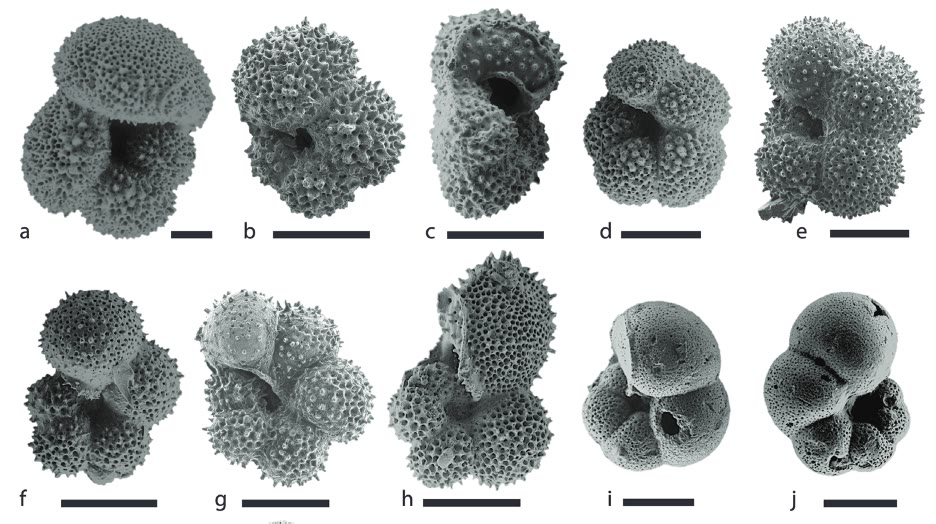
\includegraphics[width=0.62\linewidth]{images/book2/g12-planktic-foraminifera.jpg}

{\small महासागर में तैरते हुए रहने वाली फ़ोरैमिनिफ़ेरा की दस जातियों की सीपियाँ,
क्रमवीक्षण इलेक्ट्रॉन सूक्ष्मदर्शी से देखी गईं; हर मापक-पट्टी
\qty{150}{\micro\metre} की है, इसलिए हर सीपी लगभग रेत के एक कण जितनी है।
मार्सी रॉबिन्सन, USGS (सार्वजनिक डोमेन, विकिमीडिया कॉमन्स के ज़रिए)।}
\end{omfigure}
% ledger: photo:g12-forams

सीपी की ऑक्सीजन समुद्री जल से आती है। हल्के
समस्थानिक ऑक्सीजन-16 से बना जल अधिक आसानी से वाष्पित होता है, और हिमचादरें बनाने वाला
हिम इसलिए ऑक्सीजन-18 में निर्धन होता है। जब हिमचादरें बढ़ती हैं, तो वे
यह हल्का जल संचित करती हैं, और पीछे बचा महासागर ऑक्सीजन-18 में समृद्ध हो जाता है;
उसमें बढ़ने वाली सीपियाँ भी, और जल जितना ठंडा हो उतना अधिक। समुद्र-तल के
फ़ोरैमिनिफ़ेरा की सीपियों में ऑक्सीजन-18 का अंश, जिसे
$\delta^{18}\mathrm{O}$ लिखा जाता है और प्रति हज़ार भागों में दिया जाता है, इस तरह
स्थल पर बर्फ़ के आयतन और \omterm{def:g10:layered-ocean:thermocline}{गहन महासागर} के तापमान का \omterm{def:g12:past-climates:proxy}{प्रॉक्सी} है: वह
जितना ऊँचा, उतनी अधिक बर्फ़ और उतना ठंडा जल।
% ledger: nasaeo:o18, lr04:stack

नीचे का अभिलेख, जिसे LR04 कहा जाता है, सभी महासागरों के 57 कोरों के मापनों को
जोड़कर 5.3 मिलियन वर्ष का एक वक्र बनाता है।

\begin{omfigure}
\begin{tikzpicture}
\begin{axis}[omrecord, scale only axis, width=0.86\linewidth, height=4.8cm,
  xmin=0, xmax=5.32, x dir=reverse, ymin=2.4, ymax=5.3, y dir=reverse,
  xtick={0,0.5,...,5}, ytick={2.5,3,...,5},
  x tick label style={/pgf/number format/.cd, fixed, precision=1},
  y tick label style={/pgf/number format/.cd, fixed, fixed zerofill, precision=1},
  xlabel={1950 से पहले के मिलियन वर्ष},
  ylabel={सीपियों का $\delta^{18}\mathrm{O}$ (\unit{\permil})}]
\fill[omProp!14] (axis cs:1.25,2.4) rectangle (axis cs:0.7,5.3);
% data:lr04 (the stack only; ice_age_records.py)
\addplot[omDef!85!black, line width=0.35pt] table[x=age_Ma, y=d18O] {figdata/out/grade-12-ice_age_records-lr04.dat};
\addplot[omThm, line width=1pt, densely dashed, unbounded coords=jump] table[x=age_Ma, y=d18O] {figdata/out/grade-12-ice_age_records-lr04mean.dat};
\coordinate (mpt) at (axis cs:0.975,2.45);
\coordinate (mm) at (axis cs:5.22,4.92);
\coordinate (arr) at (axis cs:5.12,3.9);
\end{axis}
\node[font=\scriptsize, anchor=north, align=center] at (mpt) {41 000 से\\100 000 वर्ष};
\draw[omThm, line width=1pt, densely dashed] (mm) -- ($(mm)+(0.5,0)$) node[right, font=\scriptsize, text=omThm] {5.3 से 3 और 1 से 0 मिलियन वर्ष पहले के माध्य};
\draw[-{Stealth}, black!70] (arr) -- ++(0,-0.9) node[midway, right, font=\scriptsize, align=left] {अधिक बर्फ़,\\अधिक ठंडा};
\end{tikzpicture}

{\small समुद्र-तल के फ़ोरैमिनिफ़ेरा की सीपियों में \omterm{def:g10:layered-ocean:thermocline}{गहन महासागर} के पाँच मिलियन वर्ष;
ऊर्ध्वाधर अक्ष उलटा है, ताकि ठंडे, बर्फ़ीले समय
नीचे हों। धराशायी रेखाएँ पहले और अंतिम भागों के माध्य हैं। छायांकित:
\num{41000} वर्ष की लय से लगभग \num{100000}
वर्ष की लय में परिवर्तन। आँकड़े: लिसिएकी और रेमो (2005), LR04 संकलन।}
\end{omfigure}
% ledger: data:lr04, lr04:stack, clark06:mpt

ऊपर की विधि से पढ़ने पर, अभिलेख तीन बातें कहता है।
\begin{itemize}
  \item \emph{पृथ्वी ठंडी हुई है और उसकी बर्फ़ बढ़ी है।} माध्य मान
        5.3 और 3 मिलियन वर्ष पहले के बीच के \qty{3.03}{\permil} से
        पिछले मिलियन वर्षों में \qty{4.15}{\permil} तक उठता है।
  \item \emph{झूले बड़े हुए हैं।} हिमनदीय और अंतर्हिमनदीय समय
        पूरे अभिलेख में बारी-बारी से आते हैं, पर वे अधिकाधिक चौड़े झूलते हैं:
        \omterm{def:g12:past-climates:lgm}{अंतिम हिमनदीय अधिकतम} पर मान \qty{4.92}{\permil} था, जबकि
        आज \qty{3.23}{\permil} है।
  \item \emph{लय बदली है।} 2.6 और 1.3 मिलियन वर्ष
        पहले के बीच, अभिलेख का सबसे प्रबल आवर्तकाल, उसके आँकड़ों से परिकलित,
        \num{41000} वर्ष है; पिछले \num{700000} वर्षों में यह लगभग
        \num{98000} वर्ष है, \omterm{def:g12:past-climates:ice-core}{बर्फ़ के कोरों} की लय। परिवर्तन लगभग 1.25 और 0.7 मिलियन वर्ष पहले के
        बीच हुआ।
\end{itemize}
% ledger: data:lr04, clark06:mpt (ice_age_records.py: lr04_mean_3_5Ma 3.032, lr04_mean_0_1Ma 4.147, lr04_lgm 4.92, lr04_today 3.23, periods 41.0 and 98.5 kyr)

ये आवर्तकाल संयोग नहीं हैं। 1976 में जेम्स हेज़, जॉन इम्ब्री और निकोलस
शैकलटन ने दक्षिणी महासागरों के अवसादों में तीन लयें पाईं,
\num{23000}, \num{42000} और लगभग \num{100000} वर्ष की, जो
पृथ्वी की कक्षा और अक्ष के धीमे परिवर्तनों के आवर्तकाल हैं: अक्ष का पुरस्सरण,
अक्ष का झुकाव (लगभग \num{41000} वर्ष) और कक्षा की आकृति
(लगभग \num{100000} वर्ष)। ये परिवर्तन उस सूर्य-प्रकाश को बदलते हैं जो हर
अक्षांश को हर ऋतु में मिलता है, और वे \omterm{def:g12:past-climates:glacial-cycle}{हिमनदीय
चक्रों} की गति तय करते हैं। वे यह कैसे करते हैं, और धीमी \num{100000} वर्ष की लय क्यों
छा गई, यह विश्वविद्यालय के एक पाठ्यक्रम का विषय है।
% ledger: hays76:periods, nasa:milankovitch, lr04:stack, clark06:mpt

\begin{dated}{2025}
जनवरी 2025 में, बियॉन्ड EPICA परियोजना ने घोषणा की कि डोम~C पर
कॉनकॉर्डिया स्टेशन से लगभग \qty{35}{km} दूर, लिटिल डोम~C में ड्रिल किया गया एक कोर अपने ऊपरी
\qty{2480}{m} में लगभग 1.2 मिलियन वर्ष पीछे तक का एक सतत अभिलेख रखता है।
यह उस समय को समेटता है
जब हिमनदीय लय \num{41000} से \num{100000} वर्ष में बदली, और
बर्फ़ और उसकी वायु का विश्लेषण किया जा रहा है।
\end{dated}
% ledger: ku25:beyond-epica, ipev25:little-dome-c

\section{सुदूर अतीत की जलवायु}

\omterm{def:g12:past-climates:ice-core}{बर्फ़ के कोरों} से आगे पीछे की ओर, अतीत की जलवायु
अवसादों, जीवाश्म पत्तियों और मृदाओं, और समस्थानिकों से पढ़ी जाती है। IPCC ने कुछ
सुअध्ययित \emph{संदर्भ काल} चुने हैं, जिनकी जलवायु
आज और कल के परिवर्तनों को आँकने में सहायक है। नीचे का चार्ट उनका वैश्विक
सतह-तापमान देता है, 1850--1900 की तुलना में।

\begin{omfigure}
\begin{tikzpicture}
\begin{axis}[omrecord, width=0.86\linewidth, height=5.4cm, xmin=-9, xmax=27,
  ymin=0.4, ymax=6.6, y dir=reverse, ytick={1,...,6}, ymajorgrids=false,
  yticklabels={{PETM, 56 Ma}, {EECO, 53--49 Ma}, {MPWP, 3.3--3.0 Ma},
    {LIG, 129--116 ka}, {LGM, 23--19 ka}, {MH, 6.5--5.5 ka}},
  y tick label style={font=\scriptsize},
  xlabel={1850--1900 की तुलना में तापमान (\unit{\degreeCelsius})}]
% ipcc:fig2-34 (DEEP in ice_age_records.py)
\addplot[draw=none, mark=none, restrict expr to domain={\thisrow{tlo}}{0:30},
  error bars/.cd, x dir=both, x explicit,
  error bar style={line width=5pt, omWarm!75}, error mark=none]
  table[x expr={(\thisrow{tlo}+\thisrow{thi})/2}, y=idx,
        x error expr={(\thisrow{thi}-\thisrow{tlo})/2}] {figdata/out/grade-12-ice_age_records-deep.dat};
\addplot[draw=none, mark=none, restrict expr to domain={\thisrow{tlo}}{-30:-0.01},
  error bars/.cd, x dir=both, x explicit,
  error bar style={line width=5pt, omCold!75}, error mark=none]
  table[x expr={(\thisrow{tlo}+\thisrow{thi})/2}, y=idx,
        x error expr={(\thisrow{thi}-\thisrow{tlo})/2}] {figdata/out/grade-12-ice_age_records-deep.dat};
\draw[black!60] (axis cs:0,0.4) -- (axis cs:0,6.6);
\draw[omThm, densely dashed, line width=0.8pt] (axis cs:1.09,0.4) -- (axis cs:1.09,6.6);
\node[font=\scriptsize, text=omThm, anchor=west, fill=white, inner sep=1pt] at (axis cs:1.6,4.55) {2011--2020};
\end{axis}
\end{tikzpicture}

{\small अतीत के छह संदर्भ कालों का वैश्विक सतह-तापमान,
बहुत संभावित परास, 1850--1900 की तुलना में; धराशायी: दशक 2011--2020।
PETM: पैलियोसीन--इओसीन ऊष्मीय अधिकतम; EECO: आरंभिक इओसीन जलवायु
इष्टतम; MPWP: मध्य-प्लायोसीन गरम काल; LIG: अंतिम अंतर्हिमनदीय काल; LGM: \omterm{def:g12:past-climates:lgm}{अंतिम
हिमनदीय अधिकतम}, एकमात्र ठंडा काल (नीला); MH:
मध्य-होलोसीन। मान: IPCC AR6 WG1, चित्र 2.34।}
\end{omfigure}
% ledger: ipcc:fig2-34, ipcc:gsat-2011-2020, ipcc:ref-periods

\begin{center}
\small
\begin{tabular}{|l|c|c|c|}
\hline
\textbf{काल} & \textbf{तापमान (\unit{\degreeCelsius})} & \textbf{कार्बन डाइऑक्साइड (ppm)} & \textbf{समुद्र-तल (m)} \\
\hline
PETM, 56 Ma & $+10$ से $+25$ & लगभग 900, बढ़कर 2000 & --- \\
EECO, 53--49 Ma & $+10$ से $+18$ & 1150 से 2500 & $+70$ से $+76$ \\
MPWP, 3.3--3.0 Ma & $+2.5$ से $+4.0$ & 360 से 420 & $+5$ से $+25$ \\
LIG, 129--116 ka & $+0.5$ से $+1.5$ & 266 से 282 & $+5$ से $+10$ \\
\textcolor{omCold}{LGM, 23--19 ka} & \textcolor{omCold}{$-7$ से $-5$} & \textcolor{omCold}{188 से 194} & \textcolor{omCold}{$-134$ से $-125$} \\
MH, 6.5--5.5 ka & $+0.2$ से $+1.0$ & 260 से 268 & $-3.5$ से $+0.5$ \\
\hline
\end{tabular}

\medskip
{\small संदर्भ काल: 1850--1900 की तुलना में वैश्विक सतह-तापमान,
कार्बन डाइऑक्साइड, और 1900 की तुलना में वैश्विक समुद्र-तल। IPCC
AR6 WG1, चित्र 2.34।}
\end{center}
% ledger: ipcc:fig2-34

पैलियोसीन--इओसीन ऊष्मीय अधिकतम एक आकस्मिक तापन था, जब कार्बन का एक बड़ा
स्पंद महासागर और वायु तक पहुँचा: महासागर अधिक अम्लीय
और ऑक्सीजन में निर्धन हो गया, और गहरे समुद्र की कई जातियाँ विलुप्त हो गईं। आरंभिक इओसीन
जलवायु इष्टतम में, कार्बन डाइऑक्साइड कई मिलियन वर्षों तक \qty{1000}{ppm} से ऊपर
बनी रही, कोई ध्रुवीय बर्फ़ नहीं थी, और लगभग उष्णकटिबंधीय वन
\ang{70} दक्षिण पर उगते थे। मध्य-प्लायोसीन गरम काल वह अंतिम समय है जब कार्बन
डाइऑक्साइड आज के निकट थी: आर्कटिक अब से कहीं अधिक गरम था, और समुद्र
ऊँचा था। अंतिम अंतर्हिमनदीय काल में, ग्रीनलैंड और पश्चिमी अंटार्कटिक हिमचादरें
छोटी थीं और समुद्र आज से ऊँचा था, और दरियाई घोड़े
ब्रिटेन में रहते थे।
% ledger: ipcc:ref-periods, ipcc:fig2-34, ipcc:mpwp-eeco

ये अभिलेखागार आज को परिप्रेक्ष्य में रखते हैं, और IPCC स्वयं यह तुलना
करता है। 2019 में वायु की कार्बन डाइऑक्साइड कम से कम दो मिलियन वर्षों में किसी भी
समय से अधिक थी (\emph{उच्च विश्वास}), और 1750 से कार्बन
डाइऑक्साइड और मीथेन की वृद्धि कम से कम \num{800000} वर्षों में हिमनदीय
और \omterm{def:g12:past-climates:glacial-cycle}{अंतर्हिमनदीय कालों} के बीच के प्राकृतिक परिवर्तनों से कहीं अधिक है (\emph{बहुत उच्च
विश्वास})। वैश्विक सतह-तापमान 1970 से उतनी तेज़ी से बढ़ा है जितना
कम से कम पिछले \num{2000} वर्षों की किसी भी दूसरी 50-वर्षीय अवधि में नहीं
(\emph{उच्च विश्वास})। दशक 2011--2020 वर्तमान \omterm{def:g12:past-climates:glacial-cycle}{अंतर्हिमनदीय काल} की सबसे गरम
शताब्दियों, लगभग \num{6500} वर्ष पहले, से अधिक गरम था, और
अंतिम अंतर्हिमनदीय काल की गरमी, लगभग \num{125000} वर्ष पहले, के निकट था
(\emph{मध्यम विश्वास})।
% ledger: ipcc:co2-ch4-800kyr, ipcc:fastest-2000yr, ipcc:co2-2myr

परिवर्तन की गति की भी तुलना की जा सकती है। 1970 से 2025 तक,
वैश्विक तापमान-अभिलेख की प्रवृत्ति \qty{0.20}{\degreeCelsius} प्रति दशक है, या
यदि यह बनी रहे तो लगभग \qty{20}{\degreeCelsius} प्रति हज़ार वर्ष; पिछले
\omterm{def:g12:past-climates:glacial-cycle}{हिमनदीय काल} से बाहर निकलने वाला तापन औसतन लगभग
\qty{0.86}{\degreeCelsius} प्रति हज़ार वर्ष था। आज के परिवर्तन के कारण,
और यह क्या बन सकता है, \cref{ch:g12:climate-change} का विषय हैं।
% ledger: data:gistemp (ice_age_records.py: rate_1970_2025_C_per_decade 0.2012), ipcc:lgm-cooling, ipcc:ref-periods

\section{अभ्यास}

\begin{exercise}[$\star$]\label{exo:g12:past-climates:1}
पद बताइए: (a) किसी अभिलेखागार में मापी गई राशि जो किसी अमापित
जलवायु-चर का स्थान लेती है; (b) किसी हिमचादर से ड्रिल किया गया बर्फ़ का बेलन;
(c) दो \omterm{def:g12:past-climates:glacial-cycle}{हिमनदीय कालों} के बीच का एक गरम अंतराल; (d) जीवाश्म पराग से अतीत की
वनस्पति को पढ़ना; (e) वह समय, लगभग \num{23000} से \num{19000}
वर्ष पहले, जब पिछली हिमचादरें सबसे बड़ी थीं।
\end{exercise}

\begin{exercise}[$\star$]\label{exo:g12:past-climates:2}
हर \omterm{def:g12:past-climates:proxy}{प्रॉक्सी} के लिए उसका अभिलेखागार बताइए, और यह कि वह किसके बारे में बताता है: (a) बुलबुलों
की वायु; (b) ओक पराग का अंश; (c) समुद्र-तल के फ़ोरैमिनिफ़ेरा की सीपियों की
ऑक्सीजन-18; (d) वृक्ष-वलयों की चौड़ाई।
\end{exercise}

\begin{exercise}[$\star$]\label{exo:g12:past-climates:3}
अंतिम विहिमनदन संक्रमण के दौरान, लगभग \num{18000} से \num{11000}
वर्ष पहले तक, समुद्र-तल लगभग \qty{-120}{m} से \qty{-50}{m} तक उठा। (a)
उठने की माध्य दर, मिलीमीटर प्रति वर्ष में, परिकलित कीजिए। (b) 2006 से 2018 तक, समुद्र-तल
\qty{3.7}{mm} प्रति वर्ष उठा। तुलना कीजिए।
\end{exercise}

\begin{exercise}[$\star$]\label{exo:g12:past-climates:4}
वैश्विक तापमान 1970 से 2025 तक \qty{0.20}{\degreeCelsius} प्रति दशक
बढ़ा। इस दर को प्रति शताब्दी और प्रति हज़ार वर्ष में व्यक्त कीजिए।
\end{exercise}

\begin{exercise}[$\star$]\label{exo:g12:past-climates:5}
हेज़, इम्ब्री और शैकलटन ने समुद्री अवसादों में तीन लयें पाईं:
\num{23000}, \num{42000} और लगभग \num{100000} वर्ष। (a) हर एक को
अक्ष के पुरस्सरण, अक्ष के झुकाव और कक्षा की आकृति से मिलाइए।
(b) \num{1000000} वर्षों में \num{41000} वर्ष के कितने चक्र समाते हैं?
\num{100000} वर्ष के कितने चक्र?
\end{exercise}

\begin{exercise}[$\star\star$]\label{exo:g12:past-climates:6}
अध्याय की न्यूनतम-वर्ग रेखा $\mathrm{CO_2} \approx 266.6 +
7.83\,\Delta T$ है (ppm में, $\Delta T$ को \unit{\degreeCelsius} में लेकर)।
(a) डोम~C पर \omterm{def:g12:past-climates:lgm}{अंतिम हिमनदीय अधिकतम} के माध्य तापमान,
\qty{-9.4}{\degreeCelsius}, के लिए कार्बन डाइऑक्साइड का पूर्वानुमान कीजिए, और इसकी तुलना मापे गए
\qty{190}{ppm} से कीजिए। (b) सबसे गरम बिंदु, \qty{+5.5}{\degreeCelsius}, के लिए इसका पूर्वानुमान कीजिए,
और इसकी तुलना सबसे ऊँचे मापे गए मान, \qty{299}{ppm}, से कीजिए। (c) रेखा का उपयोग
करके डोम~C का वह तापमान आँकिए जो \qty{427}{ppm} के साथ जाता, जो मौना लोआ पर
2025 का मान है। रेखा का यह अंतिम उपयोग उचित क्यों नहीं है?
\end{exercise}

\begin{exercise}[$\star\star$]\label{exo:g12:past-climates:7}
वार्डन पहाड़ियों की झील का \omterm{def:g12:past-climates:pollen}{पराग-आरेख} उपयोग कीजिए। (a) \qty{580}{cm} पर प्रमुख
पराग कौन-सा है, और वह किस भूदृश्य को दर्शाता है? (b) यही
प्रश्न \qty{340}{cm} पर। (c) ठंड के बाद कौन-सा पेड़ पहले फैलता है, और
कौन-से पेड़ सबसे बाद में आते हैं? (d) किसी पेड़ का आगमन उस तापन से पीछे क्यों रह सकता है
जिसने उसे संभव बनाया?
\end{exercise}

\begin{exercise}[$\star\star$]\label{exo:g12:past-climates:8}
उसी कोर में, \qty{600}{cm} पर कीचड़ \num{14000} वर्ष पुराना है और
\qty{300}{cm} पर \num{6000} वर्ष पुराना, निक्षेपण की स्थिर दर के साथ।
(a) यह दर मिलीमीटर प्रति वर्ष में परिकलित कीजिए। (b) क्षेत्र 2 और 3 के बीच की
सीमा की आयु ज्ञात कीजिए, जो \qty{470}{cm} पर है। (c) \qty{1}{cm} मोटी परत
कितने वर्षों का प्रतिनिधित्व करती है?
\end{exercise}

\begin{exercise}[$\star\star$]\label{exo:g12:past-climates:9}
दक्षिण-पूर्व एशिया के मानचित्र पर, समुद्र को \qty{130}{m} नीचे करने पर समुद्र के ऊपर की भूमि 4.11 से
बढ़कर 7.16 मिलियन वर्ग किलोमीटर हो जाती है।
(a) वृद्धि और उसका प्रतिशत परिकलित कीजिए। (b) मानचित्र पर, लगभग
\qty{36}{m} की गिरावट बोर्नियो को एशिया से जोड़ने के लिए पर्याप्त है। क्या पूरे \omterm{def:g12:past-climates:lgm}{अंतिम
हिमनदीय अधिकतम} के दौरान द्वीप जुड़ा रहा? समझाइए। (c) मानचित्र की तटरेखा केवल
अनुमानित क्यों है?
\end{exercise}

\begin{exercise}[$\star\star$]\label{exo:g12:past-climates:10}
LR04 अभिलेख में, \omterm{def:g12:past-climates:lgm}{अंतिम हिमनदीय अधिकतम} पर मान
\qty{4.92}{\permil} है और आज का \qty{3.23}{\permil}। (a) कौन-सा अधिक है,
और क्या आप यही अपेक्षा करते हैं? हिमचादरों के आधार पर समझाइए। (b) अभिलेख का
ऊर्ध्वाधर अक्ष उलटा क्यों खींचा गया है?
\end{exercise}

\begin{exercise}[$\star\star$]\label{exo:g12:past-climates:11}
एक मित्र कहता है: ``अंटार्कटिक तापमान और कार्बन डाइऑक्साइड के बीच 0.92 का सहसंबंध
सिद्ध करता है कि कार्बन डाइऑक्साइड ने हिमयुगों को नियंत्रित किया।''
(a) सहसंबंध क्या दिखाता है, और क्या नहीं दिखाता? (b) दो
अन्य व्याख्याएँ दीजिए जो वही सहसंबंध देतीं। (c) दोनों अभिलेखों के बारे में किस प्रकार की
जानकारी निर्णय में सहायक होगी?
\end{exercise}

\begin{exercise}[$\star\star\star$]\label{exo:g12:past-climates:12}
LR04 अभिलेख का सबसे प्रबल आवर्तकाल 2.6
और 1.3 मिलियन वर्ष पहले के बीच \num{41000} वर्ष है, और पिछले \num{700000}
वर्षों में \num{98500} वर्ष। (a) हर खिड़की में कितने चक्र हैं? (b) पृथ्वी की
कक्षा या अक्ष का कौन-सा परिवर्तन हर आवर्तकाल से मेल खाता है? (c) समझाइए कि
हर \num{2000} वर्ष पर एक नमूने वाला अभिलेख ये लयें क्यों दिखा सकता है, पर एक शताब्दी तक चला
परिवर्तन क्यों नहीं।
\end{exercise}

\begin{exercise}[$\star\star\star$]\label{exo:g12:past-climates:13}
1995--2014 में कार्बन डाइऑक्साइड के बढ़ने की दर 192 से \qty{198}{ppm} प्रति शताब्दी
थी। पैलियोसीन--इओसीन ऊष्मीय अधिकतम के दौरान यह 4 से
\qty{42}{ppm} प्रति शताब्दी थी, और अंतिम विहिमनदन संक्रमण के दौरान अधिक से अधिक
लगभग \qty{10}{ppm} प्रति शताब्दी। (a) हाल की वृद्धि
अंतिम विहिमनदन की सबसे तेज़ वृद्धि से कितने गुना तेज़ थी? (b) PETM के सबसे धीमे और
सबसे तेज़ अनुमानों से? (c) PETM की वृद्धि लगभग 900 से लगभग
\qty{2000}{ppm} तक गई। \qty{42}{ppm} प्रति शताब्दी पर इसमें कितना समय लगता,
और आज की दर पर?
\end{exercise}

\begin{exercise}[$\star\star\star$]\label{exo:g12:past-climates:14}
IPCC का आकलन है कि अंतिम विहिमनदन के सबसे तेज़ भाग में वैश्विक तापमान 1 से
\qty{1.5}{\degreeCelsius} प्रति हज़ार वर्ष बढ़ा, और
ग्रीनलैंड के ऊपर सबसे तीव्र तापन की शताब्दियों में यह लगभग दस गुना तेज़ी से बढ़ा।
(a) ग्रीनलैंड की दर \unit{\degreeCelsius} प्रति हज़ार वर्ष और प्रति दशक में
दीजिए। (b) इसकी तुलना \qty{0.20}{\degreeCelsius} प्रति दशक की
आज की वैश्विक दर से कीजिए। (c) किसी स्थानीय दर की तुलना सीधे किसी वैश्विक दर से
क्यों नहीं करनी चाहिए?
\end{exercise}

\begin{exercise}[$\star\star\star$]\label{exo:g12:past-climates:15}
\num{11000} वर्ष पहले समुद्र-तल लगभग \qty{-50}{m} था; मान लीजिए कि वह फिर
\qty{12}{m} प्रति हज़ार वर्ष की स्थिर दर से उठा, जो मुख्य
विहिमनदन की माध्य दर है। (a) उसने \qty{-36}{m}, वह स्तर जो मानचित्र पर बोर्नियो को
एशिया से जोड़ता है, कब पार किया? (b) उस समय के बाद, क्या कोई व्यक्ति बोर्नियो से
मलय प्रायद्वीप तक पैदल जा सकता था? (c) यदि समुद्र उसी गति से उठता रहता, तो उसे अंतिम
\qty{36}{m} उठने में कितना समय लगता?
\end{exercise}

\begin{problem}[{सप्ताहांत समस्या --- अंटार्कटिक बर्फ़ के 800 000 वर्ष}]
\label{pb:g12:past-climates:1}
% ledger: data:edc-jouzel, data:co2-bereiter, data:lr04, data:gistemp, ipcc:lgm-cooling, ipcc:ref-periods, hays76:periods, clark06:mpt
% values (ice_age_records.py): edc -10.58 / +5.46, co2 173.71 / 298.6, r 0.9165, fit 266.57 + 7.827 T,
% LGM -9.389 / 189.67, 11-9 ka -0.360 / 264.10, period 97.5, rate 0.2012 per decade, ratio 23.48
डोम~C की बर्फ़ और उसके बुलबुलों की वायु निम्नलिखित मान देती हैं।
तापमान बर्फ़ के ऊपर पिछले हज़ार वर्षों की तुलना में परिवर्तन है।

\begin{center}
\small
\begin{tabular}{|l|c|c|}
\hline
 & \textbf{तापमान-परिवर्तन (\unit{\degreeCelsius})} & \textbf{कार्बन डाइऑक्साइड (ppm)} \\
\hline
सबसे ठंडा मान, लगभग \num{24000} वर्ष पहले & $-10.6$ & --- \\
सबसे गरम मान, लगभग \num{129000} वर्ष पहले & $+5.5$ & --- \\
सबसे कम और सबसे अधिक कार्बन डाइऑक्साइड & --- & 174 और 299 \\
माध्य, \num{23000} से \num{19000} वर्ष पहले & $-9.4$ & 190 \\
माध्य, \num{11000} से \num{9000} वर्ष पहले & $-0.4$ & 264 \\
\hline
\end{tabular}
\end{center}

तापमान-अभिलेख का सबसे प्रबल आवर्तकाल लगभग \num{98000} वर्ष है,
और मानों के 1639 जोड़े 0.92 का सहसंबंध गुणांक देते हैं।

\medskip
\noindent\textbf{भाग I --- दोनों अभिलेखों को पढ़ना।}
\begin{enumerate}
  \item बर्फ़ का कौन-सा भाग तापमान दर्ज करता है, और कौन-सा
        कार्बन डाइऑक्साइड?
  \item डोम~C पर तापमान-परिवर्तन का पूरा परास परिकलित कीजिए।
  \item कार्बन डाइऑक्साइड का पूरा परास परिकलित कीजिए।
  \item 0.92 का सहसंबंध गुणांक दोनों अभिलेखों के बारे में क्या
        बताता है?
  \item अध्याय के समय-अक्ष वाले चित्र में आज दाईं ओर है। ऐसा चित्र पढ़ने से पहले
        आपको यह क्यों जाँचना चाहिए कि समय किस ओर चलता है?
\end{enumerate}

\medskip
\noindent\textbf{भाग II --- हिमनदीय और अंतर्हिमनदीय मान।}
\begin{enumerate}[resume]
  \item \omterm{def:g12:past-climates:glacial-cycle}{हिमनदीय काल} और \omterm{def:g12:past-climates:glacial-cycle}{अंतर्हिमनदीय काल} की परिभाषा दीजिए।
  \item हम दोनों में से किसमें रहते हैं, और कब से?
  \item \num{800000} वर्षों में \num{98000} वर्ष के कितने चक्र समाते हैं?
  \item पृथ्वी की कक्षा के किस परिवर्तन का आवर्तकाल
        \num{100000} वर्ष के निकट है?
  \item लगभग 1.25 मिलियन वर्ष पहले से पहले, \omterm{def:g12:past-climates:glacial-cycle}{हिमनदीय चक्रों} की मुख्य लय
        क्या थी?
\end{enumerate}

\medskip
\noindent\textbf{भाग III --- अंतिम विहिमनदन।}
\begin{enumerate}[resume]
  \item \omterm{def:g12:past-climates:lgm}{अंतिम हिमनदीय अधिकतम} और \num{11000} से \num{9000} वर्ष पहले के बीच
        डोम~C के ऊपर तापमान कितना बढ़ा?
  \item उसी अंतराल में कार्बन डाइऑक्साइड कितनी बढ़ी?
  \item \omterm{def:g12:past-climates:lgm}{अंतिम हिमनदीय अधिकतम} का वैश्विक तापमान 1850--1900 के तापमान से 5 से
        \qty{7}{\degreeCelsius} कम था। इस परास का मध्य
        लीजिए। अंटार्कटिक परिवर्तन बड़ा है या छोटा?
  \item अंतिम विहिमनदन संक्रमण \num{18000} से
        \num{11000} वर्ष पहले तक चला। यह कितना समय है?
  \item संक्रमण के दौरान वैश्विक तापन की माध्य दर,
        \unit{\degreeCelsius} प्रति हज़ार वर्ष में, परिकलित कीजिए।
  \item इस दर को \unit{\degreeCelsius} प्रति दशक में व्यक्त कीजिए।
\end{enumerate}

\medskip
\noindent\textbf{भाग IV --- आज की दर से तुलना।}
\begin{enumerate}[resume]
  \item 1970 से 2025 तक वैश्विक तापमान
        \qty{0.20}{\degreeCelsius} प्रति दशक बढ़ा। इस दर को प्रति
        हज़ार वर्ष में व्यक्त कीजिए।
  \item आज का तापन अंतिम विहिमनदन के माध्य तापन से कितने गुना
        तेज़ है?
  \item विहिमनदन के सबसे तेज़ भाग में, वैश्विक तापमान
        1 से \qty{1.5}{\degreeCelsius} प्रति हज़ार वर्ष बढ़ा। आज की दर
        इनसे कितने गुना तेज़ है?
  \item निष्कर्ष निकालिए: आज का वैश्विक तापन पिछले हिमयुग से बाहर निकलने वाले तापन से
        कितने गुना तेज़ है?
\end{enumerate}
\end{problem}
